\section{FlashAttention}

\begin{frame}{FlashAttention: The Core Idea}
    \begin{itemize}\itemsep0.4em
        \item Standard attention writes the full $N \times N$ score matrix to GPU main memory (HBM), reads it back for the softmax, then reads it again to multiply with $V$: most of the time goes to memory traffic, not math.
        \item On-chip SRAM is roughly an order of magnitude faster than HBM but only megabytes in size (on an A100, about 19\,TB/s across $\sim$20\,MB of SRAM against 1.5--2.0\,TB/s across 40--80\,GB of HBM).
        \item FlashAttention (Dao et al., 2022) splits $Q$, $K$, $V$ into tiles that fit in SRAM and computes attention block by block with a running softmax, never materializing the $N \times N$ matrix.
        \item The output is exact (no approximation), memory grows linearly instead of quadratically with sequence length, and wall-clock time drops because IO shrinks.
    \end{itemize}
\end{frame}

\begin{frame}{FlashAttention: Memory Hierarchy and Tiling}
    \centering
    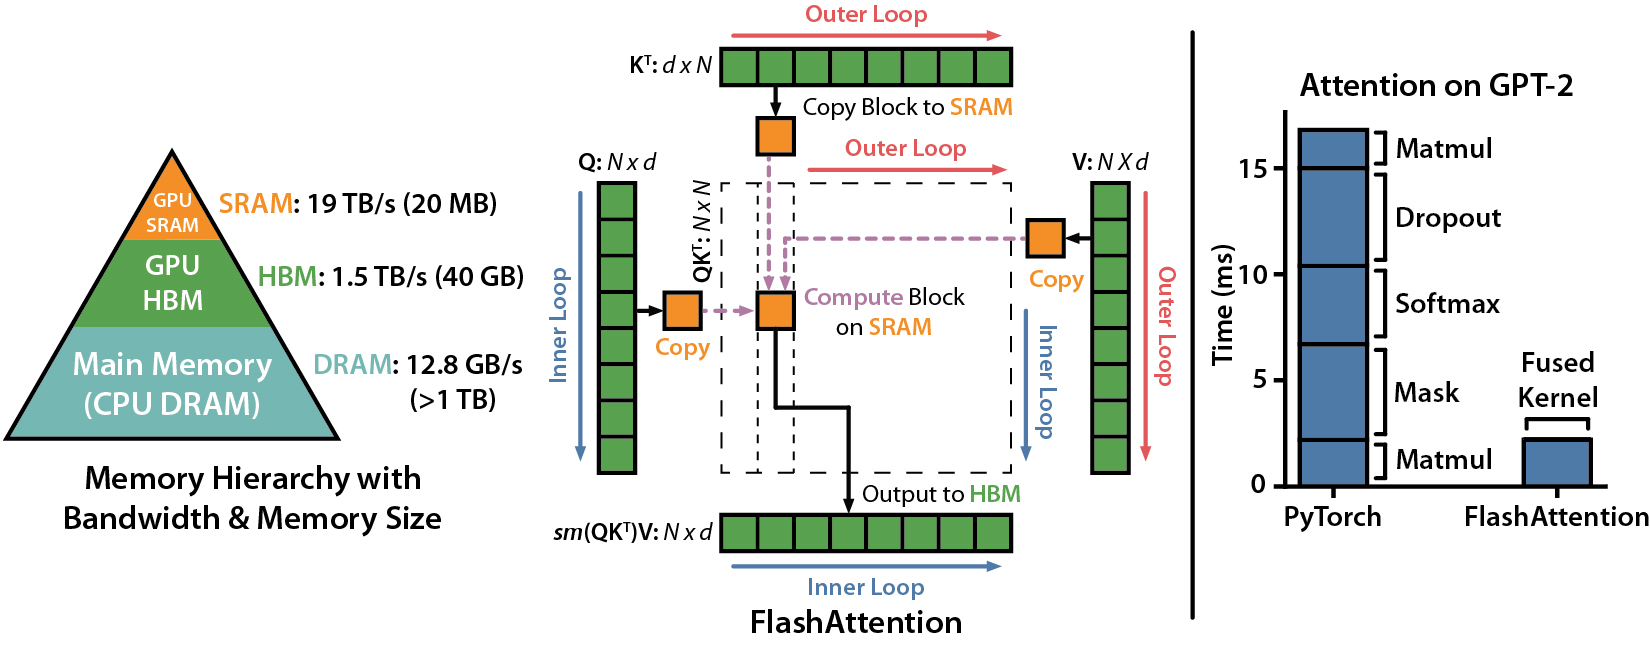
\includegraphics[width=\textwidth,height=0.72\textheight,keepaspectratio]{images/transformers-2017-v-2026/flashattention_gpu_memory_hierarchy_tiling.jpg}\\[0.3em]
    {\scriptsize GPU memory hierarchy, tiling scheme, and GPT-2 kernel timings. Dao et al., ``FlashAttention: Fast and Memory-Efficient Exact Attention with IO-Awareness,'' \href{https://arxiv.org/abs/2205.14135}{arXiv:2205.14135}; figure from the \href{https://github.com/Dao-AILab/flash-attention}{official flash-attention repository}.}
\end{frame}

\begin{frame}{FlashAttention-2: Overview}
    \begin{itemize}
        \item \textbf{Paper:} Tri Dao (2023), \href{https://arxiv.org/abs/2307.08691}{arXiv:2307.08691}
        \item \textbf{Highlights:}
        \begin{itemize}
            \item 50--73\% of theoretical peak FLOPs/s on A100, against 25--40\% for FlashAttention-1
            \item Around 2$\times$ faster than FlashAttention-1, itself 2--4$\times$ faster than optimized standard attention
        \end{itemize}
        \item \textbf{Techniques:}
        \begin{itemize}
            \item Fewer non-matmul FLOPs
            \item Parallelism over sequence length, not only batch and heads
            \item Work partitioning across warps to cut shared-memory traffic
        \end{itemize}
        \item \textbf{Adoption:}
        \begin{itemize}
            \item Widely used in open training and serving stacks (Mistral among them)
            \item The payoff is context length: 16k-context training at the price of 8k
        \end{itemize}
    \end{itemize}
\end{frame}


\begin{frame}[allowframebreaks]{FlashAttention-2: Key Improvements}
    \begin{itemize}
        \item \textbf{Fewer non-matmul FLOPs:}
        \begin{itemize}
            \item Algorithm tweaks reduce non-matmul operations (e.g., rescaling, masking).
            \item Maximizes use of specialized GPU units (Tensor Cores).
            \item Non-matmul FLOPs are up to 16$\times$ more expensive than matmul FLOPs.
        \end{itemize}
        \item \textbf{Better Parallelism:}
        \begin{itemize}
            \item Parallelizes over sequence length in addition to batch size and heads.
            \item Improves GPU utilization for long sequences and small batches.
        \end{itemize}
    \framebreak
        \item \textbf{Improved Work Partitioning:}
        \begin{itemize}
            \item Splits Q across warps (instead of K/V), reducing shared memory communication.
            \item Yields significant speedup by minimizing synchronization.
        \end{itemize}
        \item \textbf{New Features:}
        \begin{itemize}
            \item Supports head dimensions up to 256 (FlashAttention-1 stopped at 128).
            \item Supports multi-query and grouped-query attention, so kernel speed and a smaller cache combine.
        \end{itemize}
    \end{itemize}
\end{frame}

\begin{frame}[allowframebreaks]{FlashAttention-2: Tiling and Work Partitioning}
    \begin{figure}
        \centering
        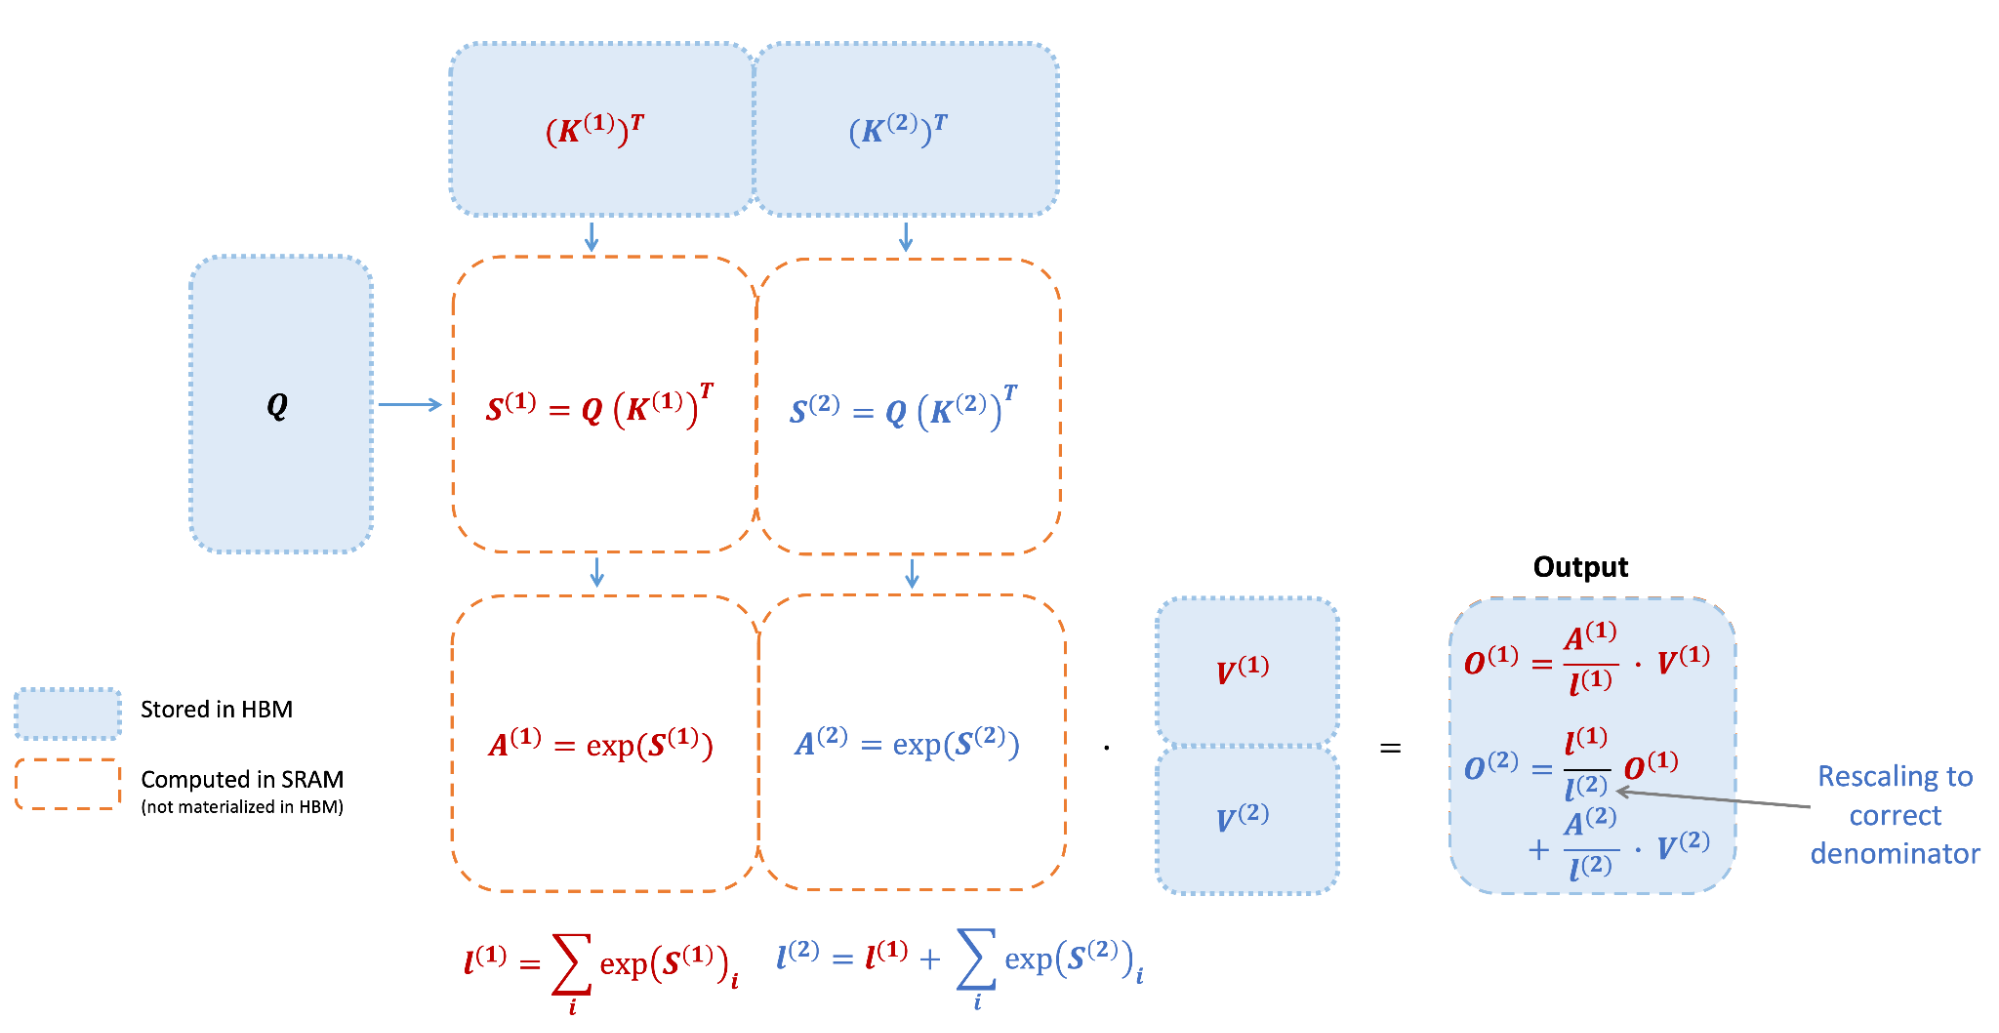
\includegraphics[height=0.80\textheight,width=\textwidth,keepaspectratio]{images/recent-advance/flash-attention-2-arch.png}
        \caption*{\scriptsize Tiled forward pass: attention is computed against one $K$/$V$ block at a time and the output rescaled to the correct denominator, so the $N \times N$ matrix never reaches HBM. Dao, ``FlashAttention-2,'' \href{https://arxiv.org/abs/2307.08691}{arXiv:2307.08691}, Figure~1.}
    \end{figure}
\framebreak
    \begin{figure}
        \centering
        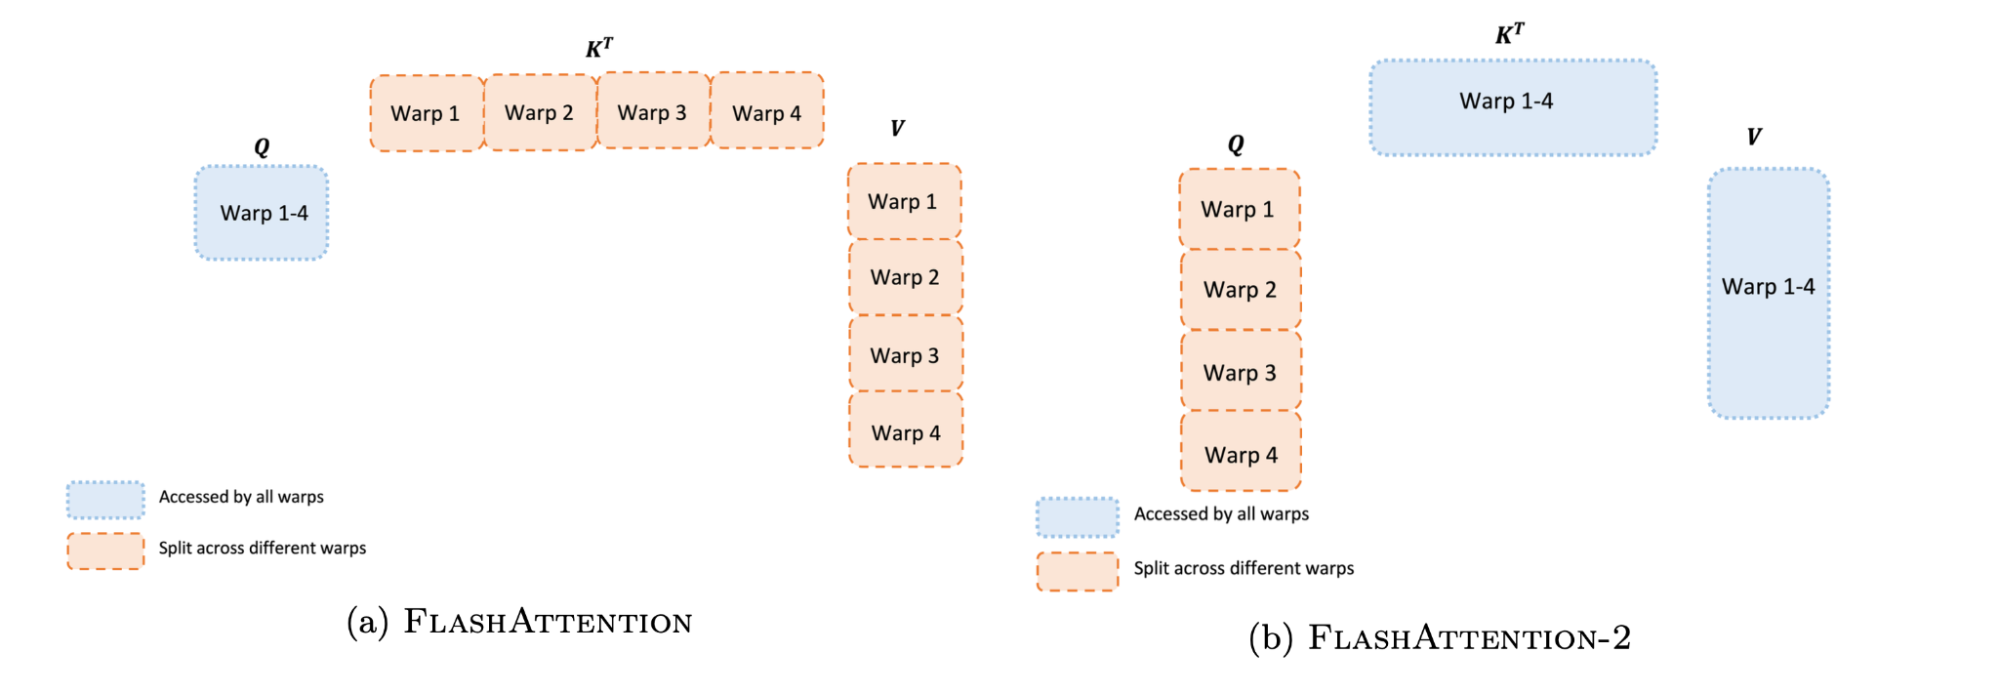
\includegraphics[height=0.80\textheight,width=\textwidth,keepaspectratio]{images/recent-advance/flash-attention-2.png}
        \caption*{\scriptsize Work partitioning between warps in the forward pass. FlashAttention-1 (a) splits $K$ and $V$ across warps and must combine partial results through shared memory; FlashAttention-2 (b) splits $Q$ instead, so no warp-to-warp communication is needed. Dao, ``FlashAttention-2,'' \href{https://arxiv.org/abs/2307.08691}{arXiv:2307.08691}, Figure~3.}
    \end{figure}
\end{frame}

\begin{frame}{FlashAttention-2: Performance Benchmarks}
    \begin{itemize}
        \item \textbf{Speed:}
        \begin{itemize}
            \item Up to 2$\times$ faster than FlashAttention-1, 9$\times$ faster than standard PyTorch attention.
            \item Up to 230 TFLOPs/s on A100 and 335 TFLOPs/s on H100.
        \end{itemize}
        \item \textbf{End-to-End Training:}
        \begin{itemize}
            \item 1.3$\times$ speedup over an already FlashAttention-optimized model.
            \item Up to 225 TFLOPs/s per A100 (72\% model FLOPs utilization).
        \end{itemize}
        \item \textbf{Example Results} (training speed, TFLOPs/s per GPU on 8$\times$A100)\textbf{:}
            \begin{tabular}{lccc}
                \toprule
                Model & Baseline & FlashAttention & FlashAttention-2 \\
                \midrule
                GPT3-1.3B 2k & 142 & 189 & 196 \\
                GPT3-1.3B 8k & 72 & 170 & 220 \\
                GPT3-2.7B 2k & 149 & 189 & 205 \\
                GPT3-2.7B 8k & 80 & 175 & 225 \\
                \bottomrule
            \end{tabular}
        \item[] {\footnotesize Baseline: Megatron-LM without FlashAttention. Dao, \href{https://arxiv.org/abs/2307.08691}{arXiv:2307.08691}, Table 1.}
    \end{itemize}
\end{frame}
